%!TEX root = ../Masterthesis.tex
\chapter{System conception}\section{Technical conception}
The technical components of the setup are relatively simple.Instead of using one large dimensioned unit which takes care of all calculations, the image processing steps that have to be done on both stereo images anyway, are outsourced onto the Raspberry Pi's.
The image processing can be done on the two Pi's in parallel, which cuts down processing time. Furthermore the image data stays on the device and does not have to be sent to a main unit which would introduce network and data reading latency.\\
The two \textbf{Raspberry Pi 3 Model B} ( Model 3 with 1GB RAM and a 64GB microSD Card running a current Raspbian OS and a C++14 compiler ), which are used as the controllers for the \textbf{Raspberry Pi Camera} are connected to the "Master"PC unit via a network Switch. The "Master" takes care of the stereoscopic calculations. The 2D positional data from the slaves and the calculation results from the stereo image disparity is fed into the hand model running on the "Master". The model solution is then applied to the digital hand model and rendered.
\section{Construction Details}
For the prototype construction, a seated use case is chosen.The tracking volume that needs to be accomplished for a seated position is limted by our physical limitations of the arm length. A tracking volume of about $100x100x100$ cm should be sufficient to track most of the movement. A seated usecase also benefits the camera system, as this needs to be calibrated for a certain depth to attain correct depth measurements.
A simple holder plate was constructed digitally and printed with a 3D Printer. Cut-outs in the mounting plate for the cameras provide the ability to mount the cameras with two machine screws and move their end position along a fixed axis. This ensures that the cameras are mounted wthout axis offsets. It furthermore give the opportunity to change the inter-axial distance of the cameras if needed. For the current setup this distance will be set to 75 mm which corresponds to the inter-axial distance of the human eyes.\\As tracking features for the position calculation, colored markers for the fingers are chosen. To ensure a natural haptic feedback, glove based solutions are not valuable. The fingers are instead painted with acrylic colors.A sixth color marker has to be positioned at the connection point between hand and forearm to serve as a global position reference
\\For the object racking part, a \textit{HTC vive marker} and \textit{Lighthouse} is used. The lighthouse is able to precisely track the position of the tracker in 3D space. The tracker can then be attached to any object that needs to be tracked.
The Raspberry's communicate with the main unit via simple UDP protcol over a local network connection.
\section{Image analysis on the Raspberry}
For the image analysis part, \textit{OpenCV3}is chosen. 
The prototype program running on the Raspberry's for tracking the specified color markers is comprised of an image acquisition stage, followed by image optimization and binary mask filtering. The resulting mask-filtered images are used for color contour finding and position calculation.\\
To reduce image analysis times a \textit{region of interest (ROI)} is defined for each marker after their successful detection. The selection of an appropriate ROI is crucial as it has to incorporate the possibility of large position differences between consecutive frames.
First frame ROI calculation is based on a minimum \textit{axis-aligned bounding box(AABB)} fitted onto the marker. The offset value from the image origin for the ROI is added to the bounding box values resulting in a rectangle data-set containing the position of the offset top-left corner $\vec{\mathbf{tl}}$ and the offset \textbf{width} and \textbf{height} of the ROI rectangle.
These values are taken to extract the sub-region of the consecutive at $\vec{\mathbf{tl}}$ with size of width and height. The $\vec{\mathbf{tl}}$ value is also saved as offset value $\vec{\mathbf{OffPos}}$ .\\The resulting rectangle has to be fitted onto the size boundaries of the full image frame by clamping the combination of position, width, height and offset to fit into the available image data boundaries.
Should no marker be found in the defined ROI the frame has to be dropped and the next frame should utilize the whole image data.\\
To compensate for white balance shifting, a non-white ideally diffuse reflecting background should be used for the tracking space and the auto modes should be turned off. Appropriate values for white balance and exposure have to be determined at the initialization step of the system. A Gaussian filter is applied to the masks which acts as a low pass filter for the image. After this step an erosion and a dilation\cite[chapter~3.11-12]{Davies.2017} is applied to the image to further eliminate unwanted noise.
On the cleaned masks, a search for the white areas whch represent the target is done. Under the assumption that all other parasitic objectshave been removed from the image, the marker should be the largest area of positive pixels in the mask frame. This area is taken as the desired tracking marker and the ROI is calculated.
\subsection{RECIEVER SIDE CALCULATIONS}
\begin{figure}[ht]
\label{fig:reciever_side_calculations} 
\centering
	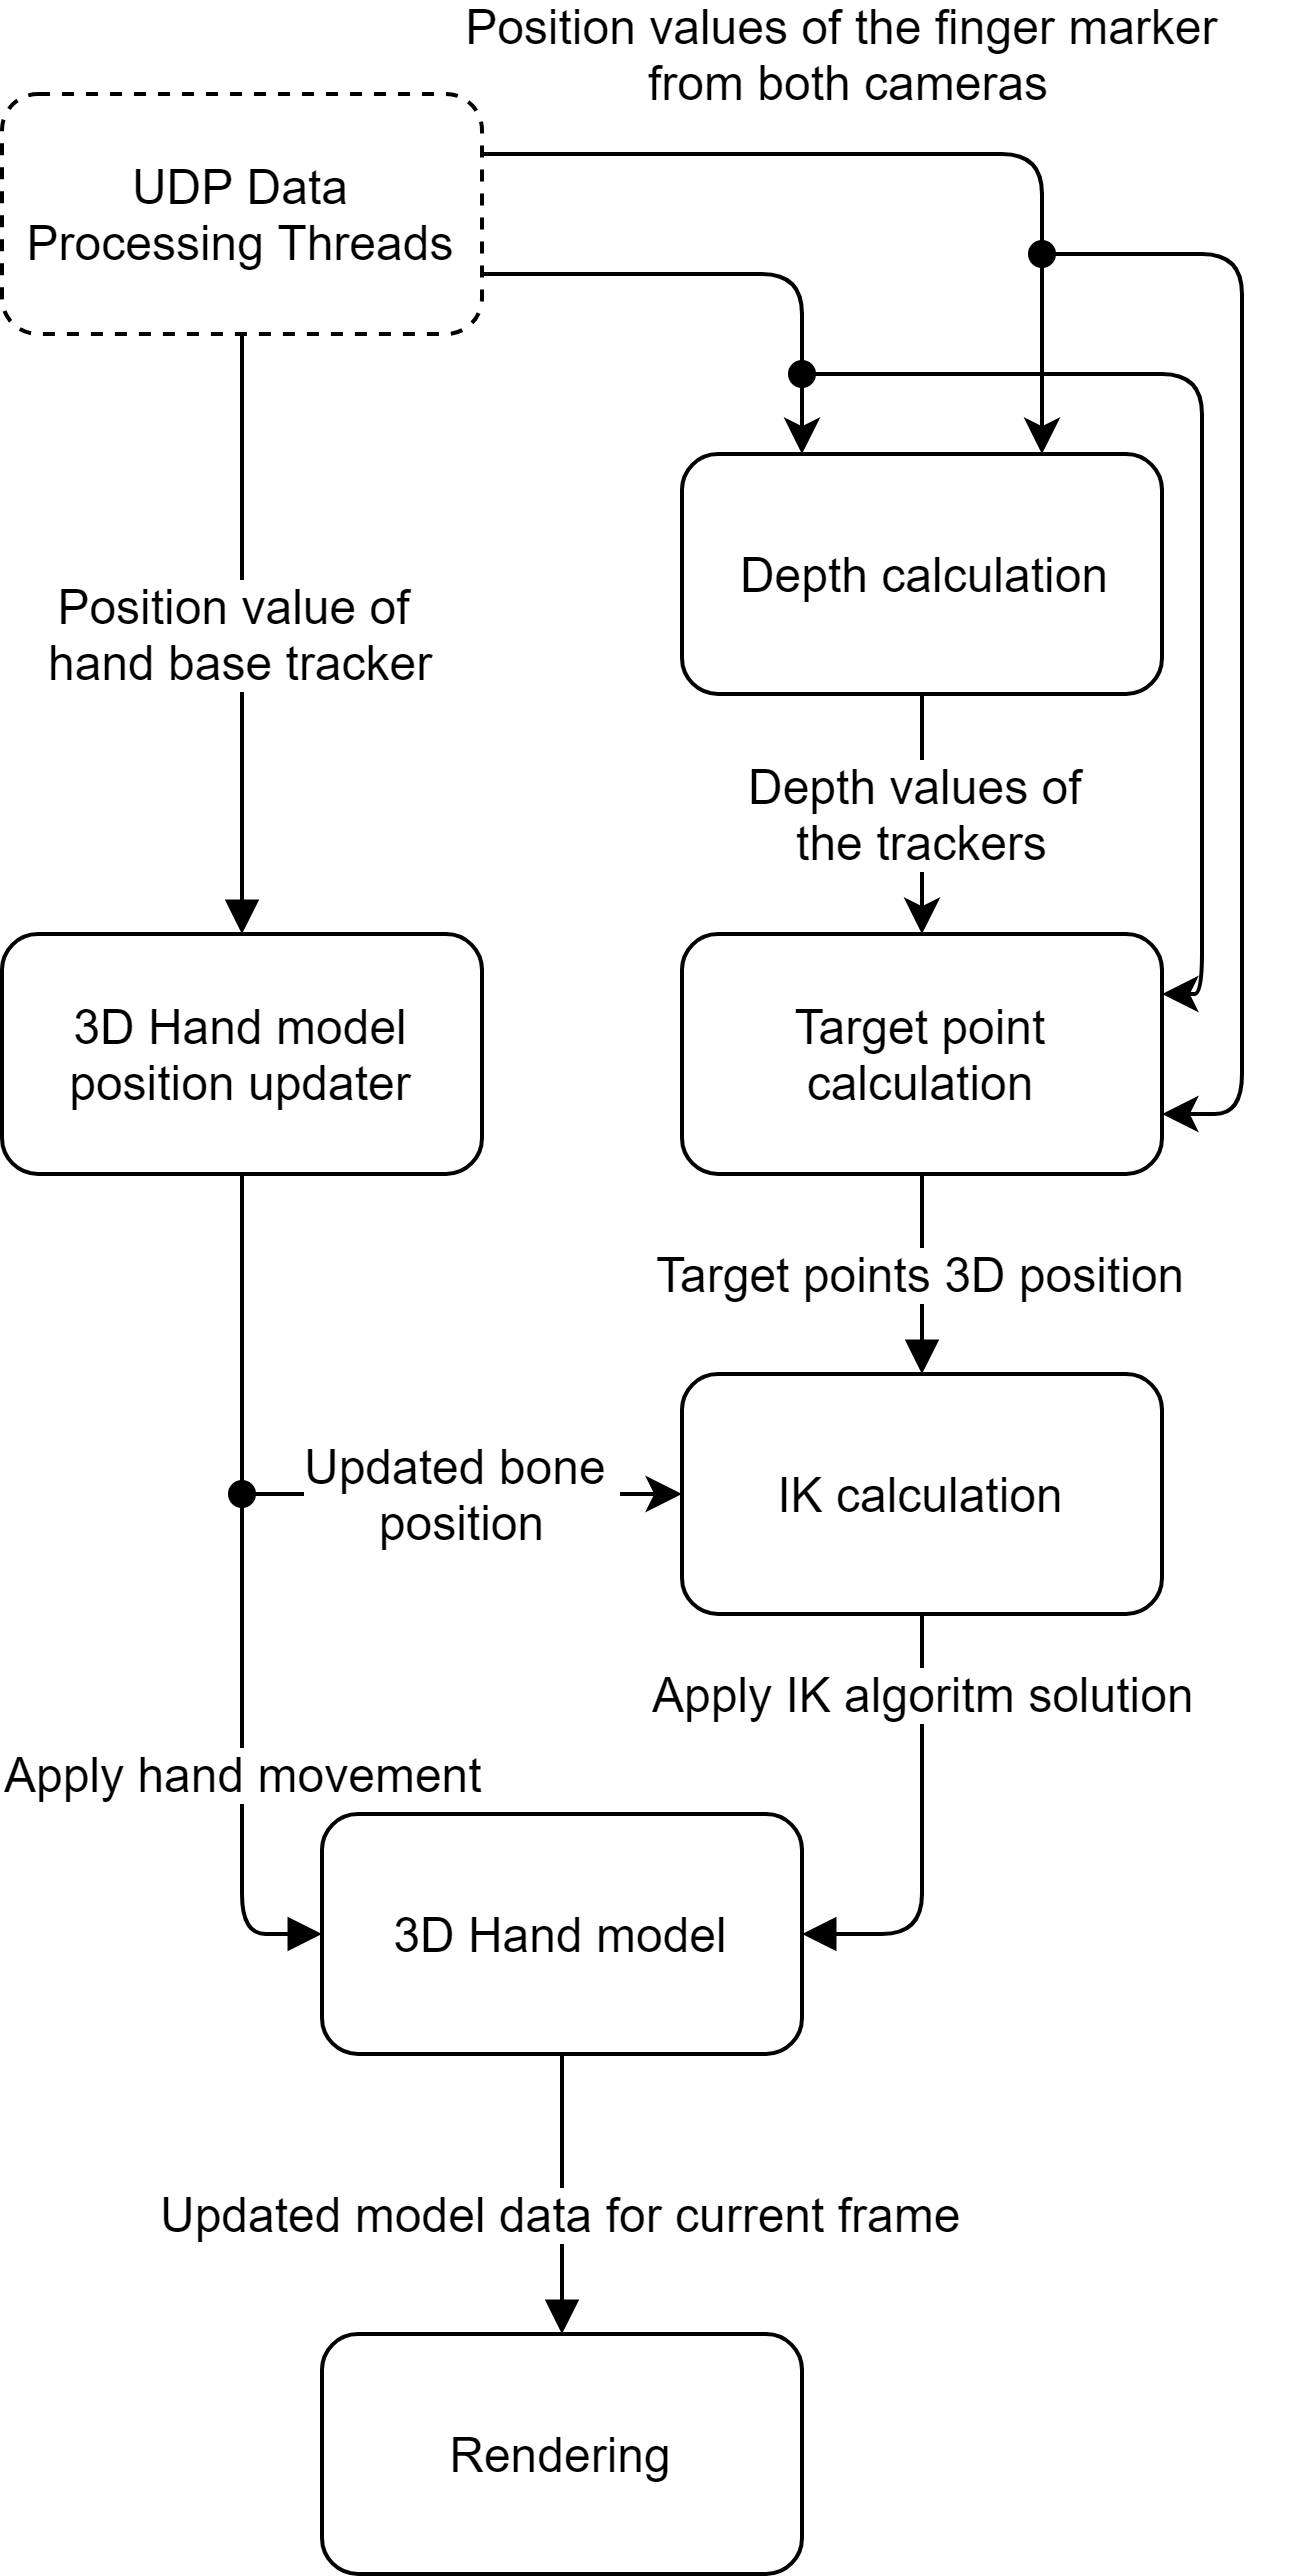
\includegraphics[width=\columnwidth/2]{images/Rendering_workflow.png}
	\caption{Workflow of the reciever side calculations}
\end{figure}
Figure \ref{fig:reciever_side_calculations} displays the workflow on the "Master" side. The UDP datastreams are processed to retrieve the 2D Position points. These are fed into the depth calculation which measures the disparity between left and right side image to calculate a depth value\cite{JernejMrovlje.2008,YasirDawoodSalman.2017,Tauer.2010}. The resulting 3D datapoints are then used to update the hand model and target points in 3D space. The IK algorithm takes the target points and tries to solve for their position.The tracked object data, which is not displayed here also gets processed and the representing digital models position gets updated before the rendering step.
\subsection{IK CALCULATION}
For the inverse kinematics calculation, the \textit{Fabrik} algorithm is used. It does not require complex matrix calculations and has a fast convergence rate. For the implementation of the algorithm on the client side, the \textit{Caliko} Java framework\cite{Lansley.2016} is used. 
For the inverse kinematics calculation to work properly the updated bone positions and the calculated target points from the finger tracking are needed.
For each finger a kinematic chain is set up with the correct bone length. The length of each bone has to be measured manually for the first prototype. The movement of each bone in the kinematic chains has to be restricted by constraints to restrict the algorithms solutions to physiological possible hand poses.  